\RequirePackage[orthodox]{nag}
\documentclass[11pt]{article}

%% Define the include path
\makeatletter
\providecommand*{\input@path}{}
\g@addto@macro\input@path{{include/}{../include/}}
\makeatother

\usepackage{../../include/akazachk}


\title{ECH4905 ChemE Optimization HW 3}
\author{Andres Espinosa}

\begin{document}
\maketitle

\section{Problem 1}
Consider the nonlinear program
\begin{align*}
  \text{minimize} & \quad x_1^2 + 2x_2^2 \\
  \text{subject to} & \quad x_1^2 + x_2^2 \leq 5 \\
  & \quad 2x_1 - 2x_2 = 1
\end{align*}

\subsection{Part a}
Write the KKT conditions for the problem
\label{p1:kkt}

\textbf{Solution: }
The KKT conditions must satisfy stationarity, complementary slackness, primal feasibility, and dual feasibility.
In order to find these conditions, we calculate the following gradients for the stationarity condition
\begin{align*}
  \nabla f_0(\textbf{x}) =
  \begin{bmatrix}
    2x_1 \\ 4x_2
  \end{bmatrix}
  , \quad
  \nabla f_1(\textbf{x}) = 
  \begin{bmatrix}
    2x_1 \\ 2x_2
  \end{bmatrix}
  , \quad
  \nabla g(\textbf{x}) = 
  \begin{bmatrix}
    2 \\ -2
  \end{bmatrix}
\end{align*}

The KKT conditions are then

\begin{align*}
  \begin{bmatrix}
    2x_1 \\ 4x_2
  \end{bmatrix}
  +
  \lambda
  \begin{bmatrix}
    2x_1 \\ 2x_2
  \end{bmatrix}
  +
  \nu
  \begin{bmatrix}
    2 \\ -2
  \end{bmatrix}
  = \textbf{0}
  & \quad \text{Stationarity} \\
  \lambda (x_1^2 + x_2^2 - 5) = 0 
  & \quad \text{Complementary Slackness} \\
  x_1^2 + x_2^2 - 5 \leq 0, \quad 2x_1 - 2x_2 - 1 = 0
  & \quad \text{Primal Feasibility} \\
  \lambda \geq 0 
  & \quad \text{Dual Feasibility}
\end{align*}

\subsection{Part b}
Using \ref{p1:kkt} and other conditions for optimality, what can you conclude about the following solutions to the nonlinear program
\begin{align*}
  \textbf{x} = 
  \begin{bmatrix}
    0 \\ 0
  \end{bmatrix}
  , \quad
  \textbf{x} = 
  \begin{bmatrix}
    1 \\ \frac{1}{2}
  \end{bmatrix}
  , \quad 
  \textbf{x} = 
  \begin{bmatrix}
    \frac{1}{3} \\ -\frac{1}{6}
  \end{bmatrix}
\end{align*}

\textbf{Solution: }
For the first point, $\textbf{x} = [0,0]$, the primal feasibility is violated because $2(0) - 2(0) -1 \neq 0$.
Therefore, this point is not feasible in the original problem and therefore not optimal.

For the second point, $\textbf{x} = [1, \frac{1}{2}]$, the following are the KKT conditions
\begin{align*}
  \begin{bmatrix}
    2 \\ 2
  \end{bmatrix}
  +
  \lambda
  \begin{bmatrix}
    2 \\ 1
  \end{bmatrix}
  +
  \nu
  \begin{bmatrix}
    2 \\ -2
  \end{bmatrix}
  = \textbf{0}
  & \quad \text{Stationarity} \\
  \lambda (1 + \frac{1}{4} - 5) = 0 
  & \quad \text{Complementary Slackness} \\
  1 + \frac{1}{4} - 5 \leq 0, \quad 2 - 1 - 1 = 0
  & \quad \text{Primal Feasibility} \\
  \lambda \geq 0 
  & \quad \text{Dual Feasibility}
\end{align*}
Since $\lambda=0$ due to the complementary slackness condition, the stationary condition is not satisfied.

For the third point, $\textbf{x} = [\frac{1}{3}, -\frac{1}{6}]$, the following are the KKT conditions
\begin{align*}
  \begin{bmatrix}
    \frac{2}{3} \\ -\frac{2}{3}
  \end{bmatrix}
  +
  \lambda
  \begin{bmatrix}
    \frac{2}{3} \\ -\frac{1}{3}
  \end{bmatrix}
  +
  \nu
  \begin{bmatrix}
    2 \\ -2
  \end{bmatrix}
  = \textbf{0}
  & \quad \text{Stationarity} \\
  \lambda (\frac{1}{9} + \frac{1}{36} - 5) = 0 
  & \quad \text{Complementary Slackness} \\
  \frac{1}{9} + \frac{1}{36} - 5 \leq 0, \quad \frac{2}{3} + \frac{1}{3} - 1 = 0
  & \quad \text{Primal Feasibility} \\
  \lambda \geq 0 
  & \quad \text{Dual Feasibility}
\end{align*}
These conditions are satisfied with $\lambda=0, \nu=-\frac{1}{3}$.
Therefore, this point $[\frac{1}{3}, -\frac{1}{6}]$ is an optimal point to the convex optimization problem above.


\section{Problem 2}
Consider the following flowsheet:

\begin{figure}[htbp]
  \centerline{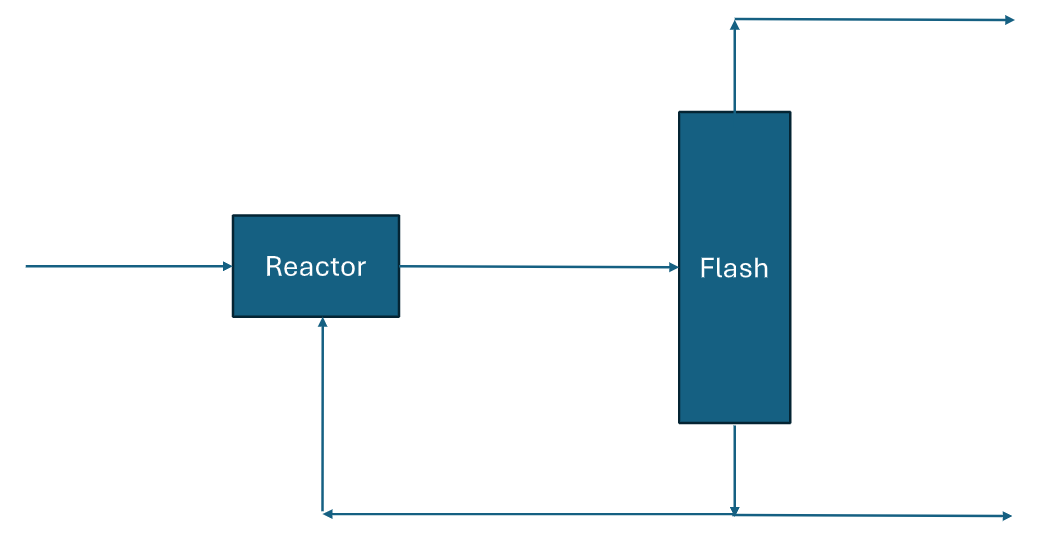
\includegraphics[width=0.5\textwidth]{images/flowsheet.png}}
  \label{fig:flowsheet}
\end{figure}

Assume that the following reaction takes place with a 50\% conversion. The feed to
the reactor consists of pure A.
\[ A \rightarrow B \]
The flash separator can be modeled as a perfect separation unit, capable of
producing any required purity.
We assume that the purge fraction should be between 1\% to 99\%.
The profit is given by the following equation:
\[ 0.5B_{\text{Top}} - 0.1F_R(500 - T) - 10^{-5}V \]
Where $B_{\text{Top}}$ is the molar flow B exiting as top product from the flash separator. 
And $F_R$ is the recycle molar flow rate.

\subsection{Part a}
Formulate a model of this process.

\textbf{Solution: }
%TODO: Formulate the model

\subsection{Part b}
Set up the model in GAMS and try 3 different NLP solvers, compare the results.

\textbf{Solution: }
%TODO: Set up the model in GAMS and compare results

\end{document}